\documentclass{bioinfo}
\copyrightyear{2021} \pubyear{2021}

%\access{Advance Access Publication Date: Day Month Year}
%\appnotes{Applications Note}

\begin{document}
%\firstpage{1}

\subtitle{GENOME ANALYSIS}

\title[StainedGlass]{StainedGlass: Making colorful dot-plots of genomic sequence}
\author[Vollger \textit{et~al}.]{
	Mitchell R. Vollger\,$^{\text{\sfb 1,}*}$,
	Peter Kerpedjiev\,$^{\text{\sfb 2}}$, 
	Adam M. Phillippy\,$^{\text{\sfb 3,*}}$, 
	and Evan E. Eichler\,$^{\text{\sfb 1,4,}*}$}
\address{
	$^{\text{\sf 1}}$Genome Sciences,
		University of Washington School of Medicine,
	 	Seattle, WA, USA \\
	$^{\text{\sf 2}}$Reservoir Genomics LLC,
	 Oakland, CA \\
	$^{\text{\sf 3}}$Genome Informatics Section,
		National Human Genome Research Institute, National Institutes of Health, Bethesda, MD, USA \\
	$^{\text{\sf 4}}$Howard Hughes Medical Institute, University of Washington, Seattle, WA, USA.
}

\corresp{$^\ast$To whom correspondence should be addressed.}

\history{}%Received on XXXXX; revised on XXXXX; accepted on XXXXX}
\editor{}%Associate Editor: XXXXXXX}

\abstract{
\textbf{Summary:} 
Visualization of genomic repeats is often accomplished through the use of 
dot plots; however, the emergence of telomere-to-telomere assemblies 
with multi-megabase repeats requires new visualization strategies. Here, 
we introduce StainedGlass which can generate publication quality figures 
that communicate the identity and orientation of 
multi-megabase repeats while scaling to entire genomes. \\
\textbf{Availability and implementation:} 
StainedGlass is implemented using \href{https://snakemake.github.io/}{snakemake}
and is available open source under the MIT license at 
\href{mrvollger.github.io/StainedGlass/}{mrvollger.github.io/StainedGlass/}.\\
\textbf{Contact:} \href{mvollger@uw.edu}{mvollger@uw.edu}\\
}

\maketitle

\section{Introduction}


\section{Usage and examples}


\citealp{Boffelli03} might want to know about  text text text text

% \begin{itemize}
% \item for bulleted list, use itemize
% \item for bulleted list, use itemize
% \item for bulleted list, use itemize\vspace*{1pt}
% \end{itemize}

% \begin{table}[!t]
% \processtable{This is table caption\label{Tab:01}} {\begin{tabular}{@{}llll@{}}\toprule head1 &
% head2 & head3 & head4\\\midrule
% row1 & row1 & row1 & row1\\
% row2 & row2 & row2 & row2\\
% row3 & row3 & row3 & row3\\
% row4 & row4 & row4 & row4\\\botrule
% \end{tabular}}{This is a footnote}
% \end{table}


\begin{figure}[!tpb]%figure1
\centerline{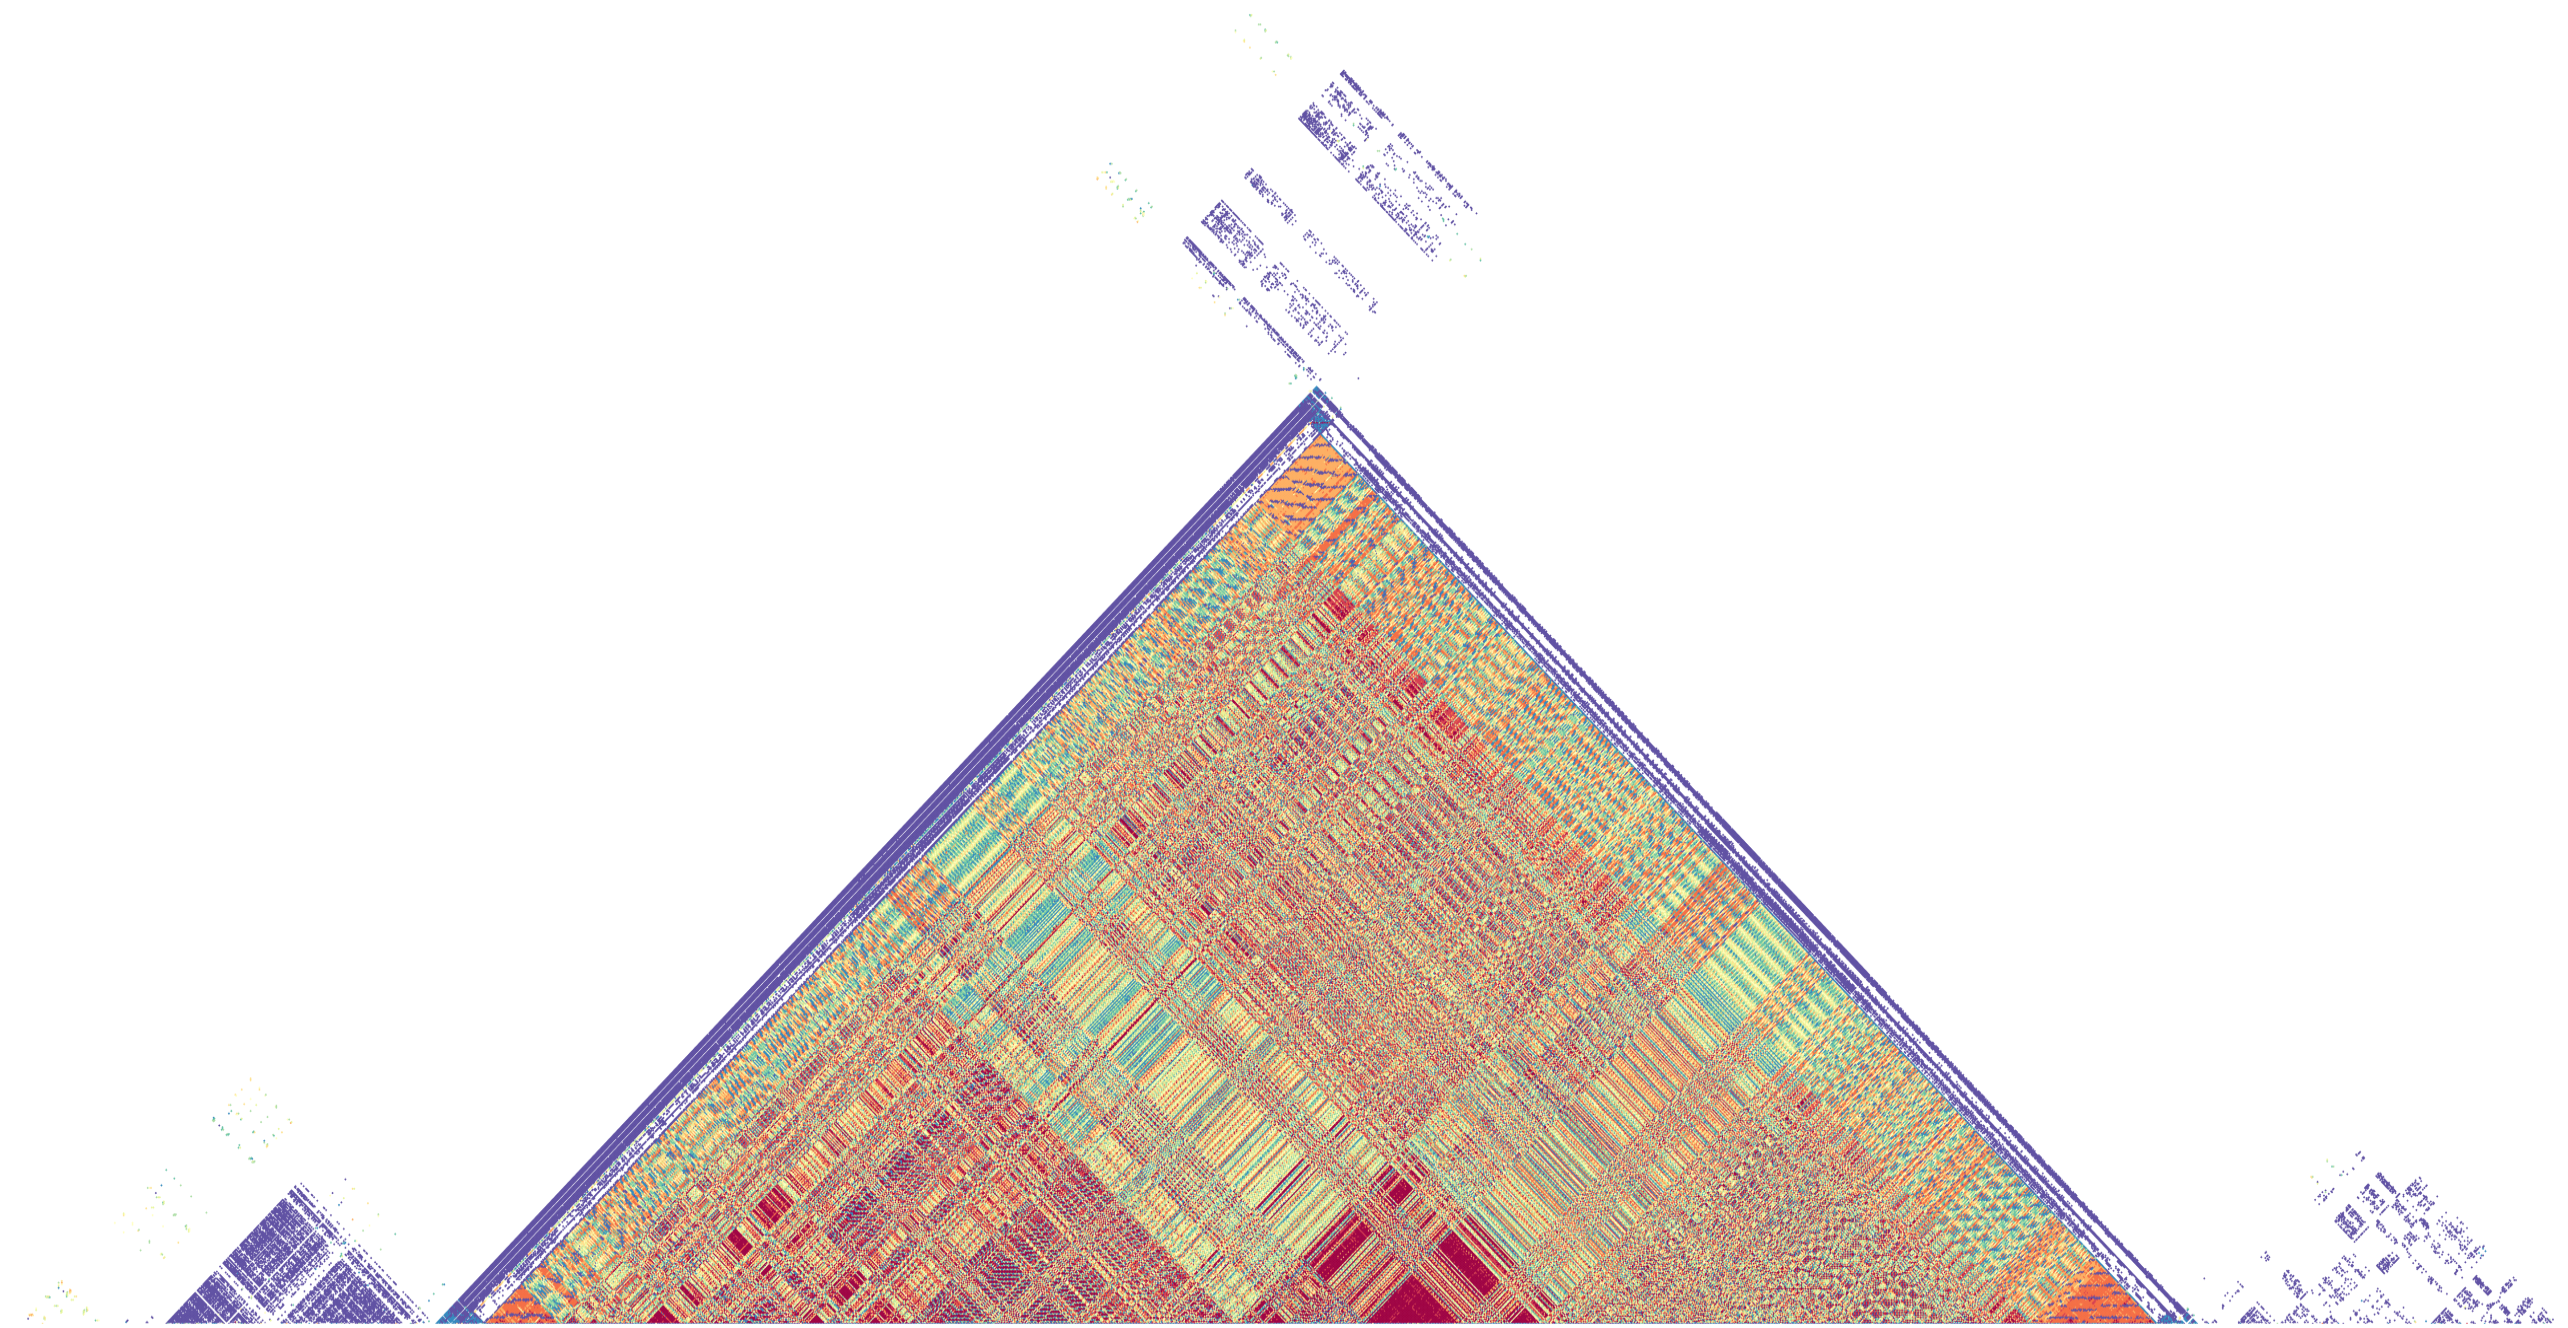
\includegraphics[width=0.5\textwidth,keepaspectratio]{../images/chr8.png}}
\caption{Caption, caption.}\label{fig:01}
\end{figure}
Figure~\ref{fig:01} 






%%%%%%%%%%%%%%%%%%%%%%%%%%%%%%%%%%%%%%%%%%%%%%%%%%%%%%%%%%%%%%%%%%%%%%%%%%%%%%%%%%%%%
%
%     please remove the " % " symbol from \centerline{\includegraphics{fig01.eps}}
%     as it may ignore the figures.
%
%%%%%%%%%%%%%%%%%%%%%%%%%%%%%%%%%%%%%%%%%%%%%%%%%%%%%%%%%%%%%%%%%%%%%%%%%%%%%%%%%%%%%%






\section{Conclusion}


\section*{Acknowledgements}

\section*{Funding}

%\bibliographystyle{natbib}
%\bibliographystyle{achemnat}
%\bibliographystyle{plainnat}
%\bibliographystyle{abbrv}
%\bibliographystyle{bioinformatics}
%
%\bibliographystyle{plain}
%
%\bibliography{Document}


\begin{thebibliography}{}

\bibitem[Bofelli {\it et~al}., 2000]{Boffelli03}
Bofelli,F., Name2, Name3 (2003) Article title, {\it Journal Name}, {\bf 199}, 133-154.


\end{thebibliography}
\end{document}
